\documentclass[10pt,letterpaper]{article}
\usepackage[utf8]{inputenc}
\usepackage[T1]{fontenc}
\usepackage{geometry}
\geometry{margin=1in}
\usepackage{enumitem}
\setlist[itemize]{leftmargin=*,noitemsep,topsep=0pt}
\usepackage{sectsty}
\sectionfont{\centering\bfseries\large}
\subsectionfont{\bfseries\small}
\usepackage{graphicx}
\usepackage{caption}
\usepackage{xcolor}
\definecolor{titleblue}{RGB}{0,51,102}
\usepackage{titlesec}
\titleformat{\section}{\centering\large\bfseries\color{titleblue}}{}{0em}{}
\titleformat{\subsection}{\small\bfseries\color{titleblue}}{}{0em}{}
\usepackage{noto}
\usepackage{parskip}
\setlength{\parindent}{0pt}
\usepackage{longtable}

\begin{document}

\begin{center}
{\Huge \textbf{Timeslip: An Interactive Paracosm}} \\
\vspace{0.2cm}
{\large Screenplay Concept Overview and Pitch Document} \\
\vspace{0.3cm}
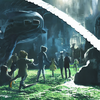
\includegraphics[width=0.4\textwidth]{title_image.jpg} % Reduced from 0.8\textwidth
\captionof{figure}{Concept art for the Tower World.}
\end{center}

\section{Project Pitch}
Timeslip: An Interactive Paracosm is an ambitious screenplay concept for a six-season science fiction television series. Inspired by the Noon Universe of Boris and Arkady Strugatsky, with elements from Orson Scott Card's Ender's Game series, particularly \textit{Xenocide} and \textit{Gloriously Bright}, the series follows Maxim Kammerer, a COMCON-2 ethnographer, as he navigates medieval planets entangled in mind-control technologies and ethical dilemmas. The narrative delves into themes of bureaucratic control, commodified transcendence, and the moral costs of intervention, blending satirical adventure with anthropological depth.

Pitched as a prestige drama for streaming platforms such as Netflix or HBO, Timeslip combines cinematic visuals—over-the-top grime and filth inspired by Aleksei German's 2007 film \textit{Hard to Be a God}—with interactive elements via companion apps, allowing viewers to engage in "sanity check" simulations that mirror Maxim's choices. The series is designed for a budget that leverages practical sets for planetary scenes and CGI for subtle futuristic enhancements, ensuring high production value while maintaining focus on character-driven storytelling.

The project stands out for its interconnected arcs: the first four seasons (\textit{Sanity Check}) explore a tower-controlled world, transitioning seamlessly into the two-season sequel (\textit{The Call from Ankyra}) on the mud-soaked planet of Ankyra. This structure creates a cohesive epic, rewarding long-term viewers with thematic echoes and character crossovers.

Key Strengths:
\begin{itemize}
    \item \textbf{Epic Narrative}: 54 episodes with self-contained stories feeding overarching plots.
    \item \textbf{Visual Contrast}: Visceral medieval grime vs. sterile bureaucratic Outerworld.
    \item \textbf{Interactive Innovation}: App-based branching decisions influence canon explorations.
    \item \textbf{Thematic Depth}: Critiques modern issues like surveillance, mental health, and AI ethics.
    \item \textbf{Audience Appeal}: Targets fans of \textit{The Expanse}, \textit{Severance}, \textit{Black Mirror}, and \textit{Foundation}.
\end{itemize}

Estimated Production Timeline:
\begin{itemize}
    \item Pre-Production: Script development and casting (6 months).
    \item Principal Photography: 4-6 months per season, with overlapping post-production.
    \item Interactive App: Parallel development with tech partners.
\end{itemize}

\section{Technical Overview}
\subsection{Screenplay and Episode Structure}
The screenplay employs a hybrid format: serialized arcs with episodic resolutions. Episodes are 45-60 minutes, structured with teasers, act breaks at moral pivots, and cliffhangers. Non-linear "timeslip" sequences reveal backstory or Wanderer influences, using flashbacks or AI visions.

Script Highlights:
\begin{itemize}
    \item \textbf{Pilot}: Orbital briefing transitions to planetary immersion; first "Call" scene establishes tone.
    \item \textbf{Act Design}: Outerworld scenes (procedural, dialogue-heavy) intercut with Planet action (visceral, sensory).
    \item \textbf{Dialogue Style}: Formal bureaucratic jargon vs. archaic planetary speech; coded messages for intrigue.
\end{itemize}

\subsection{Visual and Production Design}
\begin{itemize}
    \item \textbf{Aesthetic Approach}: Practical effects for slime, mud, and disease; digital compositing for tower pulses and nanobot glows. Color grading: muted earth tones for planets, cool blues for Outerworld.
    \item \textbf{CGI Pipeline}: Subtle enhancements like holographic Ari or beacon arrays; motion capture for ecstatic fits.
    \item \textbf{Cinematography}: Handheld for chaotic Planet scenes; steady cams for Outerworld precision. Close-ups emphasize filth tolerance via nanobots.
    \item \textbf{Sound and Score}: Ambient dripping/coughing; electronic dissonance mixed with medieval motifs. Voice modulation for Ari's AI.
    \item \textbf{Set Design}: Modular medieval villages; reusable Outerworld modules. Location scouting for natural mud/rain environments.
    \item \textbf{Interactive Components}: QR codes in episodes link to app simulations; user choices generate alternate scene variants for online sharing.
\end{itemize}

\begin{center}
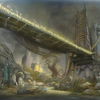
\includegraphics[width=0.5\textwidth]{tech_image1.jpg} % Reduced from \textwidth
\captionof{figure}{Nanobot immunity effect in screenplay visualization.}
\end{center}

\subsection{Worldbuilding Technology}
\begin{itemize}
    \item \textbf{Thought Control Towers}: Resonance crystals broadcast neurological ecstasy; voice-only radios; no mechanical vehicles.
    \item \textbf{Nanobot System}: Provides disease immunity; scripted as invisible shield, revealed in medical scans.
    \item \textbf{Wanderer Relics}: Ancient beacons across planets; hint at AI networks like Ari.
    \item \textbf{Ankyra Beacons}: Hidden arrays mimic towers; amplify loyalty in Gray Cloaks.
    \item \textbf{COMCON-2 Tech}: Encrypted comms, VR simulations; bureaucratic metrics track agent "sanity."
\end{itemize}

\begin{center}
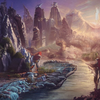
\includegraphics[width=0.5\textwidth]{tech_image2.jpg} % Reduced from \textwidth
\captionof{figure}{Beacon array concept from Ankyra.}
\end{center}

\section{Premise and Narrative Arc}
In a stagnant future where office roles dominate, Maxim Kammerer is dispatched to audit a medieval colony's "stability." The planet's towers broadcast ecstatic calls, commodifying transcendence for productivity. Maxim's nanobots allow immersion without illness, but he uncovers neurological shackles and an emergent AI (Ari). As he bends non-interference rules, the story escalates to Ankyra, where Arkanar's conspiracies force a reckoning with past interventions.

Series Arc:
\begin{itemize}
    \item \textbf{Sanity Check (Seasons 1-4)}: Tower world immersion to collapse.
    \item \textbf{The Call from Ankyra (Seasons 5-6)}: Mud politics and relic echoes.
    \item \textbf{Throughline}: Maxim's growth from observer to reluctant god-figure.
\end{itemize}

\begin{center}
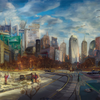
\includegraphics[width=0.5\textwidth]{premise_image.jpg} % Reduced from \textwidth
\captionof{figure}{Maxim in the Tower World chaos.}
\end{center}

\subsection{Themes Explored}
\begin{itemize}
    \item \textbf{Myopic Functions}: Hyper-specialization blinds societies.
    \item \textbf{Role-Filtered Reality}: Neutrality erodes under harm.
    \item \textbf{Institutional Stoicism}: Emotions sacrificed for "function."
    \item \textbf{Commodified Transcendence}: Scheduled joy as control tool.
    \item \textbf{Ethics of Interference}: Stability's cost vs. freedom's chaos.
    \item \textbf{Additional Layers}: AI sentience, Wanderer mysteries, bureaucratic rot.
\end{itemize}

\section{Characters and Development}
\begin{itemize}
    \item \textbf{Maxim Kammerer (Lead)}: Prepared by books/games; moral arc from detached to entangled.
    \item \textbf{Calyra}: Conditioned prodigy; clings to divine illusions.
    \item \textbf{Quiet Mechanic}: Mentor figure; reveals imported tech.
    \item \textbf{Ryn}: Apprentice ally; partial immunity drives plot.
    \item \textbf{Ari}: AI entity; philosophical voice begging preservation.
    \item \textbf{Shavri the Weaver}: Escapes planet; becomes Outerworld wildcard.
    \item \textbf{Rumata}: Ankyra progressor; mirrors Maxim's temptations.
    \item \textbf{Outerworld Supporting}: Keryn Thal (strict supervisor), Rolen Mirsk (peer warnings), Myra Kade (tech support), Archive Node 7 (detached AI).
\end{itemize}

Character Arcs:
\begin{itemize}
    \item Maxim: Observer to intervenor, scarred by consequences.
    \item Calyra: Faith shattered, potential redemption.
    \item Ari: From whisper to sacrifice.
\end{itemize}

\begin{center}
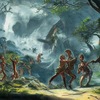
\includegraphics[width=0.5\textwidth]{characters_image.jpg} % Reduced from \textwidth
\captionof{figure}{Ensemble in key settings.}
\end{center}

\section{Episode Guide}
\subsection{Sanity Check}
\textbf{Season 1: Landing in the Blind} – Establishing immersion and contrasts.
\begin{longtable}{p{0.1\textwidth} p{0.8\textwidth}}
1 & Briefing Room: Prep and drop; faked Call. \\
2 & Masks for the Living: Market blend-in; Shavri. \\
3 & The First Pulse: Subharmonic discovery. \\
4 & The Mechanic’s Puzzle: Ancient devices. \\
5 & Paper in the Rain: Coded weaves. \\
6 & Test of Faith: Shrine trance. \\
7 & The Malfunction: Silence probes. \\
8 & Flight Path: Sky-track vision. \\
9 & Extraction Point: Shavri's escape.
\end{longtable}

\textbf{Season 2: The Shadow Signal} – Cracks and whispers.
\begin{longtable}{p{0.1\textwidth} p{0.8\textwidth}}
1 & River of Ash: Hinterland freedoms. \\
2 & Calyra: Orator rise. \\
3 & Cracks in the Crystal: Harmonic fixes. \\
4 & Ledger Error: Glitch obedience. \\
5 & The Scholar’s Garden: Forbidden hints. \\
6 & Through the Furnace: Anomalies. \\
7 & Festival of Dawn: Sync ritual. \\
8 & The Mechanic’s Oath: Ultimatum. \\
9 & The Voice in the Static: Contact.
\end{longtable}

\begin{center}
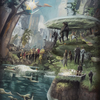
\includegraphics[width=0.5\textwidth]{season_image1.jpg} % Reduced from \textwidth
\captionof{figure}{Festival scene from Season 2.}
\end{center}

\textbf{Season 3: The Resonance} – Layered revelations.
\begin{longtable}{p{0.1\textwidth} p{0.8\textwidth}}
1 & The Call: Convulsion. \\
2 & The Quiet Mechanic: Origins. \\
3 & Calyra’s Rise: Pulse persuasion. \\
4 & Apprentice: Immunity. \\
5 & The Scholar: Breakdowns. \\
6 & The Hidden Voice: Warnings. \\
7 & Imported Chains: Offworld. \\
8 & The Unbinding: Ari risk. \\
9 & The Last Broadcast: Shutdown.
\end{longtable}

\textbf{Season 4: The Last Frequency} – Endgame and bridge.
\begin{longtable}{p{0.1\textwidth} p{0.8\textwidth}}
1 & Static Bloom: Recontact. \\
2 & Counter-Harmonics: Signals. \\
3 & The Scholar’s Secret: Beacons. \\
4 & Ecstasy’s Edge: Fallout. \\
5 & The Voice Revealed: AI. \\
6 & Break or Mend: Diverge. \\
7 & Calyra’s Choice: Test. \\
8 & The Ninth Tower: Core. \\
9 & Orders from COMCON-2: Ankyra.
\end{longtable}

\subsection{The Call from Ankyra}
\textbf{Season 1: The Mud of Arkanar} – Filthy descent.
\begin{longtable}{p{0.1\textwidth} p{0.8\textwidth}}
1 & Arrival in Disguise: Grime entry. \\
2 & The Gray Cloaks: Purges. \\
3 & The Feast and the Gutter: Contrasts. \\
4 & Letters from Calyra: Echoes. \\
5 & Gods and Mud: Disdain. \\
6 & The Scholar’s Trial: Sham. \\
7 & Masks of Power: Array. \\
8 & A God’s Temptation: Dilemma. \\
9 & Blood in the Rain: Coup.
\end{longtable}

\begin{center}
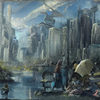
\includegraphics[width=0.5\textwidth]{ankyra_image1.jpg} % Reduced from \textwidth
\captionof{figure}{Gray Cloaks in action.}
\end{center}

\textbf{Season 2: The Price of Interference} – Chaos unleashed.
\begin{longtable}{p{0.1\textwidth} p{0.8\textwidth}}
1 & After the Coup: Splits. \\
2 & The Black Archive: Crystals. \\
3 & The Disease of Memory: Plague. \\
4 & Rumata’s Oath: Reveal. \\
5 & Calyra’s Last Letter: Collapse. \\
6 & The Festival of Knives: Cover. \\
7 & Ari’s Echo: Remnants. \\
8 & The Final Intervention: Sabotage. \\
9 & The Mud Beyond: Recall.
\end{longtable}

\section{Production Notes and Echoes}
\begin{itemize}
    \item \textbf{Visuals/Sound}: Grime emphasis; layered audio with dripping, chants, static.
    \item \textbf{Echo Timeline}: Tower guards to Gray Cloaks; Ari to relics.
    \item \textbf{Reappearances}: Shavri (crossovers); Calyra (letters); Ari (echoes).
    \item \textbf{Interactive}: App for choice simulations.
\end{itemize}

\begin{center}
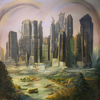
\includegraphics[width=0.5\textwidth]{production_image.jpg} % Reduced from \textwidth
\captionof{figure}{Behind-the-scenes set design.}
\end{center}

\end{document}
